\documentclass[american]{new_tlp}



\usepackage[nodate]{datetime}
\usepackage{babel}
\usepackage{amsmath}
\usepackage{mathtools}[2011/02/12]
\usepackage{amsfonts,amssymb,stmaryrd}
\usepackage{MnSymbol}
\usepackage{mdwlist}
\usepackage[applemac]{inputenc}
\usepackage{multicol}
\usepackage{galois}

\usepackage{tikz}
\usetikzlibrary{arrows}

\usepackage[linkcolor=blue, urlcolor=blue, citecolor=blue, backref=false, final]{hyperref}
\usepackage[fancyproofs,noextended,squareitemtag]{theorems}[2013/01/24]
\makeatletter
\DeclareRobustCommand{\setlabel}[1]{\def\@currentlabel{#1}}
\makeatother


\title{Abstract Diagnosis for \tccp\ using a Linear\\ Temporal Logic}

\author[M. Comini, L. Titolo and A. Villanueva]
{MARCO COMINI, LAURA TITOLO\\
DIMI, Universit\`a degli Studi di Udine, Italy\\
\email{marco.comini@uniud.it}\\
\and ALICIA VILLANUEVA 
\\
DSIC, Universitat Polit\`ecnica de Val\`encia, Spain\\
\email{villanue@dsic.upv.es}}

\providecommand*{\monobioperator}[3]{
  \newcommand*{#1}[2]{{\ifempty{##2}{#3##1}{##1#2##2}}}
}
\makeatletter
\providecommand{\ifempty}[3]{\def\@@@temp{#1}\ifx\@@@temp\@empty#2\else#3\fi}
\makeatother

\DeclarePairedDelimiterX{\mset}[2]{\langle}{\rangle}{#1\ifempty{#2}{}{\,\delimsize\vert\, #2}}
\DeclarePairedDelimiterX{\set}[2]{\{}{\}}{#1\ifempty{#2}{}{\,\delimsize\vert\, #2}}
\monobioperator{\Lconj}{\mathrel{\dot\wedge}}{\mathrel{\dot\bigwedge}}
\monobioperator{\Ldisj}{\mathrel{\dot\vee}}{\mathrel{\dot\bigvee}}
\monobioperator{\glbCC}{\sqcap}{\bigsqcap}
\monobioperator{\glbC}{\glbCsym}{\glbCbigsym}
\monobioperator{\lubCC}{\sqcup}{\bigsqcup}
\monobioperator{\lubC}{\lubCsym}{\lubCbigsym}
\newcommand*{\Aa}{\eval[]{}}
\newcommand*{\Agents}[1][\CSys]{\mathbb{A}^{\Psyms}_{#1}}
\newcommand*{\Arule}{\parensmathoper{\mathit{A}}}
\newcommand*{\Brulel}{\parensmathoper{\mathit{B}_1}}
\newcommand*{\Bruler}{\parensmathoper{\mathit{B}_2}}
\newcommand*{\CC}{\mathbb{C}}
\newcommand*{\CSdom}{\mathcal{C}}
\newcommand*{\CSfalse}{\mathit{false}}
\newcommand*{\CShid}[2]{\mathop{\exists}\nolimits_{#1} #2}
\newcommand*{\CSimp}{\mathrel{\vdash}}
\newcommand*{\CSmerge}{\mathbin{\otimes}}
\newcommand*{\CSnimp}{\mathrel{\nvdash}}
\newcommand*{\CSord}{\preceq}
\newcommand*{\CStrue}{\mathit{true}}
\newcommand*{\CSys}{\mathbf{C}}
\newcommand*{\Conf}{\mathit{Conf}}
\newcommand*{\C}[1][]{\mathbb{M}_{#1}}
\newcommand*{\Dd}{\Tp[]}
\newcommand*{\Dmst}{D_{m}}
\newcommand*{\Drc}{\{\Dmst\}}
\newcommand*{\D}{\prog}
\newcommand*{\FAa}[3][]{\mathop{\mathLTL{A}_{\mathit{#1}}}\ifempty{#2}{}{\BBrackets[{#3}]{#2}}}
\newcommand*{\FDd}[1][]{\syntaxoper{\mathLTL{D}_{\mathit{#1}}}}
\newcommand*{\FI}{\mathLTL{I}}
\newcommand*{\FSym}{\mathC{F}}
\newcommand*{\Fdom}{\mathbb{F}}
\newcommand*{\Fsyms}{\CSys,\Psyms}
\newcommand*{\FtoM}{\parensmathoper{\gamma^{\Fdom}}}
\newcommand*{\F}[2][\alpha]{\syntaxoper{\FSym^{#1}}{#2}{}}
\newcommand*{\Isym}[1]{\mathC{I}^{#1}}
\newcommand*{\I}[1][\alpha]{\Isym{#1}}
\newcommand*{\Lalways}[1]{\ifempty{#1}{\mathop{\Box}}{\mathop{\Box} #1}}
\newcommand*{\Leventually}[1]{\ifempty{#1}{\mathop{\Diamond}}{\mathop{\Diamond} #1}}
\newcommand*{\Lfalse}{\dot{\mathit{false}}}
\newcommand*{\Lhid}[2]{\mathop{\dot{\exists}}\nolimits_{#1} \ifempty{#2}{}{#2}}
\newcommand*{\Liff}[2]{\ifempty{#1}{\dot\leftrightarrow}{#1 \mathrel{\dot\leftrightarrow} #2}}
\newcommand*{\Limpl}[2]{#1 \mathrel{\dot\rightarrow} #2}
\newcommand*{\Lneg}[1]{\ifempty{#1}{\mathop{\dot{\neg}}}{\mathop{\dot{\neg}} #1}}
\newcommand*{\Lnextnum}[2]{\ifempty{#2}{\mathop{\bigcirc^{#1}}}{\mathop{\bigcirc^{#1}} #2}}
\newcommand*{\Lnext}[1]{\ifempty{#1}{\mathop{\bigcirc}}{\mathop{\bigcirc} #1}}
\newcommand*{\Lnimpl}[2]{#1 \mathrel{\dot\nrightarrow} #2}
\newcommand*{\Ltrue}{\dot{\mathit{true}}}
\newcommand*{\Luntil}[2]{\ifempty{#1}{\mathcal{U}}{#1 \mathrel{\mathcal{U}} #2}}
\newcommand*{\MGCsym}{\mathbb{PC}}
\newcommand*{\MGC}[1][]{\MGCsym_{#1}}
\newcommand*{\ProgSym}{D}
\newcommand*{\ProgsSym}{\mathbb{D}}
\newcommand*{\Progs}[1][\CSys]{\ProgsSym^{\Psyms}_{#1}}
\newcommand*{\Psyms}{\Pi}
\newcommand*{\Qq}[2]{\Q{#2}{#1}}
\newcommand*{\Q}[2]{\ifempty{#2}{#1}{#2 \mathbin{.} #1}}
\newcommand*{\SF}{\mathLTL{S}}
\newcommand*{\Ssym}[1]{\mathC{S}^{#1}}
\newcommand*{\Sz}[1][\alpha]{\Ssym{#1}}
\newcommand*{\Tbranches}{\mathit{B}}
\newcommand*{\Tinit}[1][\Phi]{n_{#1}}
\newcommand*{\Tlabel}{\parensmathoper{\mathit{L}}}
\newcommand*{\Tname}[1][\Phi]{\mathcal{T}_{#1}}
\newcommand*{\Tnodes}{\mathit{Nodes}}
\newcommand*{\TpSym}{\mathC{D}}
\newcommand*{\Tp}[3][\alpha]{\syntaxoper{\TpSym^{#1}}{#2}{{#3}}}
\newcommand*{\Tsucc}{\mathrel{\mathit{R}}}
\newcommand*{\Ttabl}[1][\Phi]{(\Tnodes, \Tinit[#1], \Tlabel{} , \Tbranches, \Tsucc{}{} )}
\newcommand*{\Var}{\mathit{Var}}
\newcommand*{\aask}[1]{\mathop{\mathsf{ask}}\ifempty{#1}{}{(#1)\ra}}
\newcommand*{\ahiding}[3][]{\mathop{\exists^{#1}{#2}} {#3}}
\newcommand*{\anowpar}[3]{\anow{(#1)}{#2}{#3}}
\newcommand*{\anow}[3]{\tagnow\ifempty{#1}{} {\: #1 \tagthen #2\ifempty{#3}{}{\tagelse #3}}}
\newcommand*{\aparallel}[2]{#1 \parallel #2}
\newcommand*{\apcall}[2]{\mathit{#1}\ifempty{#2}{}{(\mathit{#2})}}
\newcommand*{\asat}[2]{#1 \models #2}
\newcommand*{\askip}{\mathord{\mathsf{skip}}}
\newcommand*{\asumask}[4][i]{\sum_{#1=1}^{#2}\aask{#3_{#1}}{#4}_{#1}}
\newcommand*{\atell}{\parensmathoper{\mathsf{tell}}}
\newcommand*{\botCC}{\bot}
\newcommand*{\botC}{\{\ecrs\}}
\newcommand*{\botF}{\Lfalse}
\newcommand*{\call}[3]{\termres{\mathit{#1}\ifempty{#2}{}{\mathit{(#2)}}}{#3}}
\newcommand*{\ccp}{\textit{ccp}}
\newcommand*{\clauseif}{\ensuremath{\mathrel{\mathord{:}\mathord{-}}}}
\newcommand*{\closed}[1][A]{\ifempty{#1}{S}{s}elf-sufficient}
\newcommand*{\cltl}{\textsf{CLTL}}
\newcommand*{\cntx}[1]{{#1}^{*}}
\newcommand*{\cond}[2]{(#1 ,\allowbreak #2)}
\newcommand*{\controller}{master}
\newcommand*{\cpo}[2]{{(#1, \, \mathord{#2})}}
\newcommand*{\csC}[3]{\cs{\cond{#1}{#2}}{#3}}
\newcommand*{\csltl}[1][]{\ensuremath{\textsf{csLTL}_{#1}}}
\newcommand*{\cs}[2]{ #1 \rightarrowtail #2}
\newcommand*{\deffun}[1][A]{process}
\newcommand*{\dfn}{\coloneq}
\newcommand*{\ecrs}{\epsilon}
\newcommand*{\ed}{\boxtimes}
\newcommand*{\evalSym}{\mathC{A}}
\newcommand*{\eval}[4][\alpha]{\syntaxoperEXT{#3}{\evalSym^{#1}}{\termres{#3}{#2}}{#4}}
\newcommand*{\genrule}[2]{#1 \clauseif #2}
\newcommand*{\geqC}{\sqsupseteq}
\newcommand*{\glbCbigsym}{\bigsqcap}
\newcommand*{\glbCsym}{\sqcap}
\newcommand*{\glbF}{\Lconj}
\newcommand*{\interpA}[1][\A]{\mathbb{I}_{#1}}
\newcommand*{\interpF}{\interpA[\Fdom]}
\newcommand*{\latticeC}{\lattice{\C}{\leqC}{\lubC{}{}}{\glbC{}{}}{\topC}{\botC}}
\newcommand*{\latticeF}{\lattice{\Fdom}{\leqF}{\lubF{}{}}{\glbF{}{}}{\topF}{\botF}}
\newcommand*{\lattice}[6]{{(#1, \, \mathord{#2}, \, \mathord{#3}, \, \mathord{#4}, \, \mathord{#5}, \, \mathord{#6})}}
\newcommand*{\leqCC}{\sqsubseteq}
\newcommand*{\leqC}{\leqCC}
\newcommand*{\leqF}{\Limpl{}{}}
\newcommand*{\lfpof}[2][]{\mathoper{lfp}_{#1}\Braces{#2}}
\newcommand*{\lfp}[1][]{\lfpof[{#1}]{}}
\newcommand*{\ltl}{\textsf{LTL}}
\newcommand*{\lubCbigsym}{\bigsqcup}
\newcommand*{\lubCsym}{\sqcup}
\newcommand*{\lubF}{\Ldisj}
\newcommand*{\lub}{\ensuremath{\mathit{lub}}}
\newcommand*{\mathC}{\mathcal}
\newcommand*{\mgc}[4][n]{\call{#2}{\mbox{}}{#4}}
\newcommand*{\mghead}[3][n]{\mathit{#2}\ifempty{#3}{}{(\zseq[#1]{\mathit{#3}})}}
\newcommand*{\mgrule}[4][n]{\genrule{\mghead[#1]{#2}{#3}}{#4}}
\newcommand*{\nextop}{\parensmathoper{\mathsf{next}}}
\newcommand*{\nleqCC}{\nsqsubseteq}
\newcommand*{\nleqC}{\nleqCC}
\newcommand*{\nleqF}{\Lnimpl{}{}}
\newcommand*{\notasat}[2]{#1 \nmodels #2}
\newcommand*{\notsat}[2]{#1 \mathrel{\not\models} #2}
\newcommand*{\nra}{\not\rightarrow}
\newcommand*{\ntcc}{\textit{ntcc}}
\newcommand*{\phicont}{\parensmathoper{\phi_{\mathit{M}}}}
\newcommand*{\pltl}{\textsf{PLTL}}
\newcommand*{\programs}{sets of declarations}
\newcommand*{\program}{set of declarations}
\newcommand*{\progrules}{\progrule s}
\newcommand*{\progrule}{process declaration}
\newcommand*{\prog}[1][]{\ensuremath{\ProgSym_{\mathit{#1}}^{}}}
\newcommand*{\prule}[3]{\genrule{\mathit{#1}\ifempty{#2}{}{\mathit{(#2)}}}{#3}}
\newcommand*{\query}[1][A]{\ifempty{#1}{P}{p}rogram}
\newcommand*{\ra}{\rightarrow}
\newcommand*{\seqHid}[2]{\mathop{\bar{\exists}}\nolimits_{#1} #2}
\newcommand*{\seq}[2][n]{{#2}_{1}, \dots, {#2}_{#1}}
\newcommand*{\stutt}[1]{\parensmathoper{\mathit{stutt}}{#1}}
\newcommand*{\tagelse}{\mathrel{\mathsf{else}}}
\newcommand*{\tagnow}{\mathop{\mathsf{now}}}
\newcommand*{\tagthen}{\mathrel{\mathsf{then}}}
\newcommand*{\tccp}{\textit{tccp}}
\newcommand*{\tcc}{\textit{tcc}}
\newcommand*{\termres}[2]{{#1} \ifempty{#2}{}{}}
\newcommand*{\topCC}{\top}
\newcommand*{\topC}{\mathbf{M}}
\newcommand*{\topF}{\Ltrue}
\newcommand*{\zseq}[2][n]{\vec{#2}}
\newcommand{\mathLTL}[1]{\hat{\mathcal{#1}}}
\providecommand*{\BBrackets}[2][]{\ifempty{#2}{}{\llbracket#2\rrbracket_{#1}}}
\providecommand*{\Braces}[2][]{\ifempty{#2}{}{( #2 )_{#1}}}
\providecommand*{\false}{\mathit{false}}
\providecommand*{\ie}   {i.e.,} 
\providecommand*{\mathoper}[1]{\mathop{\mathit{#1}}\nolimits}
\providecommand*{\pair}[2]{{\langle #1, \, #2 \rangle}}
\providecommand*{\parensmathoper}[2]{\ensuremath{\mathoper{#1}\ifempty{#2}{}{(#2)}}}
\providecommand*{\resp} {respectively}
\providecommand*{\st}   {s.t.}
\providecommand*{\syntaxoperEXT}[4]{\mathoper{#2}\ifempty{#1}{}{\llbracket#3\rrbracket_{#4}}}
\providecommand*{\syntaxoper}[3]{\mathoper{#1}\BBrackets[#3]{#2}}
\providecommand*{\true}{\mathit{true}}
\providecommand*{\wrt}  {w.r.t.}

\newcommand*{\sequent}[4][]{\gdef\and{\quad\hfill}
    \gdef\ands{\;\hfill\ldots\hfill\;}\global\setlabel{#1}
    {#1}\frac{\:\:#2\:\:}{\;#3\;}\;\text{\small#4}}

\renewcommand*{\P}{\prog}
    


\begin{document}
\pagestyle{plain}
\maketitle
\begin{abstract}
    Automatic techniques for program verification usually suffer the
    well-known state explosion problem.  Most of the classical approaches
    are based on browsing the structure of some form of model (which
    represents the behavior of the program) to check if a given
    specification is valid.  This implies that a part of the model has to
    be built, and sometimes the needed fragment is quite huge.
    
    In this work, we provide an alternative automatic decision method to
    check whether a given property, specified in a linear temporal logic,
    is \emph{valid} \wrt\ a \tccp\ program.  Our proposal (based on
    abstract interpretation techniques) does not require to build any model
    at all.
    Our results guarantee correctness but, as usual when using an abstract
    semantics, completeness is lost.
\end{abstract}



\begin{keywords}
    concurrent constraint paradigm, 
    linear temporal logic, 
    abstract diagnosis,
    decision procedures,
    program verification
\end{keywords}

\section{Introduction}




The Concurrent Constraint Paradigm (\ccp, \cite{Saraswat89phd}) is a
simple, logic model which is different from other (concurrent) programming
paradigms mainly due to the notion of store-as-constraint that replaces the
classical store-as-valuation model.  It is based on an underlying
constraint system that handles constraints on variables and deals with
partial information.  Within this family, \cite{deBoerGM99} introduced the
\emph{Timed Concurrent Constraint Language} (\tccp\ in short) by adding to
the original \ccp\ model the notion of time and the ability to capture the
absence of information.  With these features, one can specify behaviors
typical of reactive systems such as \emph{timeouts} or \emph{preemption}
actions.




It is well-known that modeling and verifying concurrent systems by hand can
be an extremely hard task.  Thus, the development of automatic formal
methods is essential.  One of the most known techniques for formal
verification is model checking, that was originally introduced in
\cite{ClarkeE81,QueilleS82} to automatically check if a finite-state system
satisfies a given property.  It consisted in an exhaustive analysis of the
state-space of the system; thus the state-explosion problem is its main
drawback and, for this reason, many proposals in the literature try to
mitigate it.






All the proposals of model checking have in common that a \emph{part} of
the model of the (target) \query\ has to be built, and sometimes the needed
fragment is quite huge.  In this work, we propose a completely different
approach to the formal verification of temporal (\ltl) properties of
concurrent (reactive) systems specified in \tccp.  We formalize a method to
validate a specification of the expected behavior of a \tccp\ program ,
expressed by a linear temporal formula , which does not require to
build any model at all.

The linear temporal logic we use to express specifications, \csltl, is an
adaptation of the propositional \ltl\ logic to the concurrent constraint
framework.
This logic is also used as the basis of the abstract domain for a new
(abstract) semantics for the language.

In brief, our method is an \emph{extension} of abstract diagnosis for
\tccp\ \cite{CominiTV11absdiag} where the abstract domain  is formed
by \csltl\ formulas.  We cannot use the original abstract diagnosis
framework of \cite{CominiTV11absdiag} since  is not a complete
lattice.



The contributions of this work are the following:
\begin{itemize}
    
    \item 
    A new abstract semantics for \tccp{} programs based on \csltl{}
    formulas;
    
    \item 
    A novel and effective method to validate \csltl{} properties based on
    the ideas of abstract diagnosis.  This proposal intuitively consists in
    viewing  as a formula transformer by means of an (abstract)
    immediate consequence operator  which works on \csltl\
    formulas.  Then, to decide the validity of , we just have to
    check if  (\ie\ the -transformation of )
    implies ;
    
    \item 
    An automatic decision procedure for \csltl{} properties that makes our
    method effective.
\end{itemize}

With our technique we can check, for instance, that, at a railway crossing
system, each time a train is approaching, the gate is down, or that
whenever a train has crossed, the gate is up.  When a property is non
valid, the method identifies the buggy \progrule.  Technical results of
Sections~\ref{sec:CLTLabstr} and~\ref{sec:abs-diag} can be found in
\cite{CominiTV14-techrep}.


\section{The small-step operational behavior of the \tccp\ language}
\label{sec:Sem}

The \tccp{} language \cite{deBoerGM99} is particularly suitable to specify
reactive and time critical systems.  As the other languages of the \ccp{}
paradigm \cite{Saraswat93}, it is parametric \wrt\ a \emph{cylindric
constraint system} which handles the data information of the program in
terms of constraints.  The computation progresses as the concurrent and
asynchronous activity of several agents that can accumulate information in
a \emph{store}, or query information from it.  Briefly, a cylindric
constraint system\footnote{See \cite{deBoerGM99,Saraswat93} for more
details on cylindric constraint systems.} is an algebraic structure  composed of a set of constraints
 such that  is a complete algebraic lattice
where  is the  operator and  and  are
respectively the greatest and the least element of ;  is a
denumerable set of variables and  existentially quantifies
variables over constraints.  The \emph{entailment}  is the inverse
of .


Given a cylindric constraint system  and a set of process symbols
, the syntax of agents is given by the grammar:

where ,  are finite constraints in ; 
and  denotes a generic tuple of  variables.  A \tccp{} \query\
is an object of the form , where  is an agent, called
\emph{initial agent}, and  is a set of \emph{process declarations} of
the form  (for some agent ).  The notion of time is
introduced by defining a discrete and global clock.
\begin{figure}[t]
    \begin{minipage}{\textwidth}
        {\footnotesize
        {\setlength{\jot}{1.5ex}
        
        }
        }
        \caption[The transition system for \tccp{}.]{The transition system for \tccp{}.\footnotemark{}}
        \label{fig:op_sem}
    \end{minipage}
\end{figure}
\footnotetext{The auxiliary agent  makes explicit the
local store  of .  This auxiliary agent is linked to the principal
hiding construct by setting the initial local store to , thus
.  }


The \emph{operational semantics} of \tccp{}, defined in \cite{deBoerGM99},
is formally described by a transition system .
Configurations in  are pairs  representing the agent
 to be executed in the current global store .  The transition
relation  is the least relation
satisfying the rules of Figure~\ref{fig:op_sem}.  Each transition step takes
exactly one time-unit.
\begin{example}[Guiding example]\label{ex:gateController}
    Through the paper, we use as guiding example a part of the full
    specification of a railway crossing system introduced in
    \cite{AlpuenteGPV06}.  Let us call  the following \tccp{}
    declaration: {\small
    
    }Due to the monotonicity of the store, streams (written in a
    list-fashion way) are used to model \emph{imperative-style} variables
    \cite{deBoerGM99}.  The \controller\ process uses an \emph{input
    channel}  (implemented as a stream) through which it receives
    signals from the environment (trains), and an \emph{output channel} 
    through which it sends orders to a gate process.  It checks the input
    channel for a \textit{near} signal (the guard in the first
     agent), in which case it sends (tells) the order
    \textit{down} through , links the future values () of the stream
     and restarts the check at the following time instant (recursive
    call ).  If the \emph{near} signal is not
    detected, then, the else branch looks for the \emph{out} signal and (if
    present) behaves dually to the first branch.  Finally, if no signal is
    detected at the current time instant (last else branch), then the
    process keeps checking from the following time instant.
\end{example}

In this work, we prove the correctness of our technique \wrt\ the
denotational concrete semantics of \cite{CominiTV13semTR}, which is
fully-abstract (correct and complete) \wrt\ the small-step operational
behavior of \tccp{}.  Also \csltl{} is interpreted over this
denotational model.  We thus introduce the most relevant aspects of
such semantics.


The denotational semantics of a \tccp{} program consists of a set of
\emph{conditional (timed) traces} that represent, in a compact way, all the
possible behaviors that the program can manifest when fed with an
\emph{input} (initial store).  Conditional traces can be seen as
hypothetical computations in which, for each time instant, we have a
condition representing the information that the global store has to satisfy
in order to proceed to the next time instant.  Briefly, a conditional trace
is a (possibly infinite) sequence  of
\emph{conditional states}, which can be of three forms:
\begin{description}
    \item[conditional store:] 
    a pair , where  is a \emph{condition} and
     a store;
    
    \item[stuttering:] 
    the construct , with ;
    
    \item[end of a process:] 
    the construct .
\end{description}
Intuitively, the conditional store  means that, provided
condition  is satisfied by the current store, the computation
proceeds so that in the following time instant, the store is .  A
\emph{condition}  is a pair  where
 and  are called positive and
negative condition, \resp.  The positive/negative condition represents
information that a given store must/must not entail, thus they have to be
consistent in the sense that  .
The stuttering construct models the suspension of the computation when none
of the guards in a non-deterministic agent is satisfied.   is the set of
guards in the non-deterministic agent.  Conditional traces are monotone
(\ie\ for each  and  such that
, ) and consistent (\ie\ each store in a trace
does not entail the negative conditions of the following conditional
state).

We denote the domain of \emph{conditional trace sets} as .  
is a complete lattice, where .  We define as  the sequence resulting by removing
from  all the information about the variable .  We
distinguish two special classes of conditional traces.   is said
to be \emph{\closed} if the first condition is 
and, for each  and
,  (each store satisfies the successive condition).  Moreover,
 is \emph{-\closed} if  is \closed.
Thus, this definition demands that for \closed\ conditional traces, no
additional information (from other agents) is needed in order to
\emph{complete} the computation.\footnote{The set of all \closed\
conditional traces can be considered as a generalization (using conditional
states in place of stores) of the traditional strongest postcondition for
semantics.}


The semantics definition is based on a semantics evaluation function
 \cite{CominiTV13semTR} which, given an agent  and an
interpretation , builds the conditional traces associated to .
The interpretation  is a function which associates to each process
symbol a set of conditional traces ``modulo variance''.  The semantics for
a set of process declarations  is the fixpoint  of the continuous immediate consequences operator
.  Proof of full abstraction \wrt\ the operational
behavior of \tccp{} is given in \cite{CominiTV13semTR}.
\begin{figure}[tp]
    \centering{
    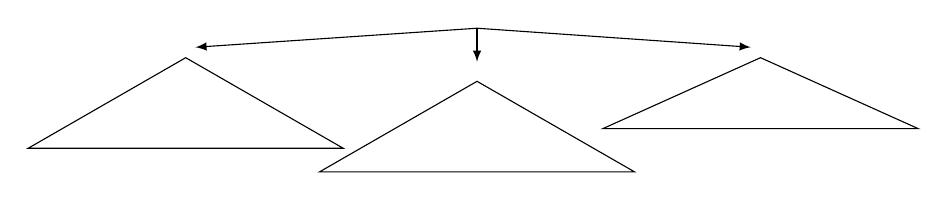
\begin{tikzpicture}[scale=0.5]
        
        \draw (0,0) coordinate (root);
        \draw (root)+(-7.4,-0.5) node (near1) {};
        \draw (root)+(0,-1.1) node (out1) {};
        \draw (root)+(7.2,-0.5) node (rec1) {};
        \draw[-latex] (root) -- (near1);
        \draw[-latex] (root) -- (out1);
        \draw[-latex] (root) -- (rec1);
        
        \draw (near1.south)+(4,-2.3) coordinate (con13);
        \draw (near1.south)+(-4,-2.3) coordinate (con14);
        \draw (near1.south) -- (con13) -- (con14) -- cycle;
        \draw (near1.south)+(0,-1.4) node (con1call)
        {\small };
        \draw (out1.south)+(4,-2.3) coordinate (con23);
        \draw (out1.south)+(-4,-2.3) coordinate (con24);
        \draw (out1.south) -- (con23) -- (con24) -- cycle;
        \draw (out1.south)+(0,-1.4) node (con2call)
        { \small };
        \draw (rec1.south)+(-4,-1.8) coordinate (con33);
        \draw (rec1.south)+(4,-1.8) coordinate (con34);
        \draw (rec1.south) -- (con33) -- (con34) -- cycle;
        \draw (rec1.south)+(0,-1.4) node (con3call) {\small};
    \end{tikzpicture}
    }
    \caption{Tree representation of   of
    \smartref{ex:TrainSmallStep}.}
    \label{fig:controllerSmallStep}
\end{figure}  
\begin{example}\label{ex:TrainSmallStep}
    Consider the \progrule{}  of \smartref{ex:gateController}.
    Given an interpretation , the semantics of
     is graphically represented in
    Figure~\ref{fig:controllerSmallStep}, where we have used some shortcuts
    for characteristic constraints.  Namely, , , , , , .
    
    The branch on the left represents the computation when a \emph{near}
    signal arrives.  The first conditional state requires that
     holds, thus the constraints  and
     are \emph{concurrently} added to the store during
    that computational step.  A recursive call is also concurrently
    invoked.  Process calls do not modify the store when invoked, but they
    affect the store from the following time instant, which is graphically
    represented by the triangle labeled with the interpretation of the
    process.  The branch in the middle is taken only if  is
    entailed and  is not entailed by the initial store (it
    occurs in the negative condition of the first conditional state in that
    branch).  Finally, the branch on the right represents the case when
    both  and  are not entailed by the
    initial store.
\end{example}

\section{Abstract semantics for \tccp\ over \csltl\ formulas} 
\label{sec:CLTLabstr}


In this section, we present a novel abstract semantics over formulas that
approximates the small-step semantics described in \smartref{sec:Sem} and,
therefore, the small-step operational behavior of a \tccp\ program.  To
this end, we first define an abstract domain of logic formulas which is a
variation of the classical Linear Temporal Logic \cite{MannaP92}.
Following \cite{PalamidessiV-CP2001,deBoerGM01,deBoerGM02,Valencia05}, the
idea is to replace atomic propositions by constraints of the underlying
constraint system.
\begin{definition}[\csltl{} formulas] \label{def:tf}
    Given a cylindric constraint system ,  and
    , formulas of the \emph{Constraint System Linear Temporal
    Logic} over  are:
    
     is the set of all temporal formulas over  (we
    omit  if clear from the context).
\end{definition}
, , , , ,
 have the classical logical meaning.  The atomic
formula  states that  has to be entailed by the current
store.   is the existential quantification over the set of
variables .  As usual, we use  as a shorthand
for ;  for
;  for
;
 for  and  for
.  A \emph{constraint formula} is an
atomic formula  or its negation .  Formulas  and
 are called \emph{next} formulas.  Constraint and next
formulas are said to be \emph{elementary} formulas.  Finally, formulas of
the form ,  or
 are called \emph{eventualities}.

We define the abstract domain  (\ie{} the
domain formed by \csltl{} formulas modulo logical equivalence) ordered by 
.
The algebraic lattice  is not complete, since both 
and  always exist just for finite sets of formulas.

The semantics of a temporal formula is typically defined in terms of an
infinite sequence of states which validates it.  Here we use conditional
traces instead.  As usually done in the context of temporal logics, we
define the satisfaction relation  only for infinite conditional
traces.  We implicitly transform finite traces (which end in ) by
replicating the last store infinite times.
\begin{definition}
    \label{def:FtoM}
    \label{def:asat}
    The \emph{semantics} of  is given by function  defined as
    ,
    where, for each ,  and
    , satisfaction relation  is defined as:
    
            &\asat{r}{\Ltrue} \quad\text{and}\quad \notsat{r}{\Lfalse}\\
            &\asat{\csC{\eta^+}{\eta^-}{d} \cdot r'}{c} &&\text{iff }
            \eta^+ \CSimp c
            \label{eq:asatKnowCS}\\
            &\asat{\stutt{\eta^-} \cdot r'}{c} &&\text{iff } \forall
            d^{-}\in \eta^- .\, c \CSnimp d^{-} \text{ and } \asat{r'}{c}
            \label{eq:asatKnowST}\\
            &\asat{r}{\Lneg{\phi}} &&\text{iff } \notasat{r}{\phi}
            \label{eq:asatNeg} \\
            &\asat{r}{\Lconj{\phi_1}{\phi_2}} &&\text{iff } \asat{r}{\phi_1}
            \text{ and } \asat{r}{\phi_2} \label{eq:asatConj} \\
            & \asat{r}{\Lnext{\phi}} &&\text{iff}\ \asat{r^1}{\phi} 
            ~\footnotemark
            \label{eq:asatNext} \\
            & \asat{r}{\Luntil{\phi_1}{\phi_2}} &&\text{iff }            
            \exists i\geq
            1 .\, \forall j < i .\ \asat{r^i}{\phi_2}\ \text{and}\ \asat{r^j}{\phi_1}
            \label{eq:asatUntil} \\
            &\asat{r}{\Lhid{x}{\phi}} 
            \quad\quad\quad\; \makebox[0pt][l]{iff exists  \st\
            ,  -\closed\ and
            }
            \label{eq:asatHid}
        \footnotetext{ denotes the sub-sequence of  starting from
    state .  }We say that  is a \emph{sound approximation} of  if .
     is said to be \emph{satisfiable} if there exists
     such that , while it is
    \emph{valid} if, for all , .
\end{definition}


All the cases are fairly standard except \eqref{eq:asatKnowCS} and
\eqref{eq:asatKnowST}.
The conditional trace  prescribes that
 is entailed by the current store, thus  models all the
constraint formulas  such that .  We have to note that,
by the monotonicity of the store of \tccp{} computations, the positive
conditions in conditional traces contains all the information previously
added in the constraint store.
Furthermore, by the definition of condition, since  cannot be in
contradiction with , it holds that neither  is in contradiction
with .  Thus, the conditional trace 
models all the constraint formulas  that are not in contradiction with
the set  and such that  holds in the continuation  by
monotonicity.
\begin{lemma}\label{lem:FtoM}
    The function  is monotonic, injective
    and -distributive.
\end{lemma}


\subsection{\csltl\ Abstract Semantics}


The technical core of our semantics definition is the \csltl\ agent
semantics evaluation function  which, given an agent  and an
interpretation  (for the process symbols of ), builds a \csltl\
formula which is a sound approximation of the (concrete) behavior of .
In the sequel, we denote by  the set of agents and  the
set of sets of process declarations built on signature  and
constraint system .
\begin{definition}
    \label{def:interpC}
    Let ,  are distinct
    variables.
    An \emph{-interpretation} is a function  modulo
    variance\footnote{\ie\ a family of elements of , indexed by
    , modulo variance.  }.  Two functions 
    are \emph{variants}
    if for each  there exists a renaming  such that
    .
    The semantic domain  is the set of all
    -interpretations ordered by the point-wise extension of .
\end{definition}    
\begin{definition}[\csltl\ Semantics]
    \label{def:semFAa} 
    Given  and , we define the \emph{\csltl\
    semantics evaluation}  by structural induction as
    follows.
    
    Given  we define the immediate consequence operator
     as
    
\end{definition}

We have that  is a sound approximation of  and
 is a sound approximation of .
\begin{theorem}[Correctness of  and ]
    \label{th:FAa_FDd_soundness}
    Let ,  and .  Then,
     and
    .
\end{theorem}
\begin{example}\label{ex:TrainAbsSem}
    Consider the \progrule{}  of \smartref{ex:gateController} and
    let us use  to abbreviate the repetition of 
    -times.
    Given , with \smartref{def:semFAa} we compute
    
    where 
    {\small
    
    }The three disjuncts of  match the three possible
    behaviors of : when signal 
    is emitted by the train, when  is emitted, and when no
    signal arrives.
\end{example}



\section{Abstract diagnosis of \tccp\ with \csltl\ formulas}
\label{sec:abs-diag}

Since  is not a complete lattice, it is impossible to find for the
function  an adjoint function  which forms a Galois
Connection , and therefore we cannot use the
abstract diagnosis framework for \tccp\ defined in
\cite{CominiTV11absdiag}.  Thus, we propose in this section a new weaker
version of abstract diagnosis that works on  \footnote{Actually, the
proposal is defined using just  only for the sake of simplicity.
It could easily be defined parametrically \wrt\ a suitable family of
concretization functions.  }.

Given a \program\  and , which is the specification
of the abstract intended behavior of  over , we say that
\begin{enumerate}
    
    \item\label{pt:COR:def:Correct}
     is (abstractly) \emph{partially correct}\index{partially correct}
    \wrt\  if .
    
    \item\label{pt:COM:def:Correct}
     is (abstractly) \emph{complete}\index{complete} \wrt\  if
    .
\end{enumerate}
The differences between  and  are usually called
\emph{symptoms}.  Many of the symptoms are just a consequence of some
``originating'' ones, those which are the direct consequence of errors.
The \emph{abstract diagnosis} determines exactly the ``originating''
symptoms and, in the case of incorrectness, the faulty \progrules\ in .
This is captured by the definitions of \emph{abstractly incorrect
\progrule} and \emph{abstract uncovered element}:\footnote{It is worth
noticing that although the notions defined in this section are similar to
those defined for the standard approach, the formal definitions and proofs
are different due to the weaker framework.}
\begin{definition}
    \label{def:ab.incorclau}
    \label{def:ab.uncovered}
    
    Let ,  a \progrule\ for \deffun[long] ,
     and .
    \begin{itemize}
        \item  is \emph{abstractly incorrect} \wrt\  (on testimony
        ) if  and
         .
        
        \item  is an \emph{uncovered element} for 
        \wrt\  if  and
        .
    \end{itemize}
\end{definition}
Informally,  is abstractly incorrect if it derives a wrong abstract
element  from the intended semantics.  Dually,  is
uncovered if the declarations cannot derive it from the intended semantics.
\begin{theorem}
    \label{th:ab.corr-compl}
    Let  and . (1)
    If there are no abstractly incorrect
    process declarations in  (\ie\ ),
    then  is partially correct \wrt\ .
    (2) If  is partially correct \wrt\  and  has abstract
    uncovered elements then  is not complete.
\end{theorem}
Absence of abstractly incorrect declarations is a sufficient condition for
partial correctness, but it is not necessary.  Because of the
approximation, it can happen that a (concretely) correct declaration is
abstractly incorrect.  Hence, abstract incorrect declarations are in
general just a warning about a possible source of errors.  However, an
abstract correct declaration cannot contain an error; thus, no (manual)
inspection is needed for declarations which are not abstractly incorrect.
Moreover, as shown by the following theorem, all concrete errors---that are
``visible''---are indeed detected, as they lead to an abstract
incorrectness or abstract uncovered.  Intuitively, a concrete error is
\emph{visible} if we can express a formula  whose concretization
reveals the error (\ie\ if the logic is expressive enough).
\begin{theorem}
    \label{th:abs-conc}
    
    Let  be a process declaration for ,  a concrete
    specification and  a sound approximation for  (\ie\ ).
    (1) If  and it exists 
    such that 
    and , then  is
    abstractly incorrect \wrt\  (on testimony ).
    (2) If there exists an abstract uncovered element  \wrt\
    , then there exists  such that .
\end{theorem}
Point~2 says that the concrete error has an abstract symptom which is not
hidden by the approximation on  and, moreover, there exists a formula
 which can express it.

In the following examples, we borrow from \cite{AlpuenteGPV06} the notation
for \emph{last entailed value} of a stream:  holds if the last
instantiated value in the stream  is .
\begin{example}\label{ex:controllDiag-validProp} 
    We verify (for \smartref{ex:gateController}) that each time a
    \emph{near} signal arrives from a train, the order \emph{down} is sent
    to a gate process.\footnote{A more interesting property, namely that,
    in addition, the gate is eventually down, is verified in
    \cite{CominiTV14-techrep}.  Here we have simplified the property due to
    space limitations.} To model this property, we define the specification
    (of the property)  as
    -5ex]
    
        \phi \dfn \SF_{\mathit{up}}(\call{\controller'}{C,G}{}) \dfn 
        \Lalways{(\Limpl{(C \dot{=} \mathit{out})} {\Leventually{(G \dot{=}
        \mathit{up}})})}
    
        \phi' \dfn \FDd{ \{R\} }{\SF_\mathit{up}} (\call{\controller'}{C,G}{}) =
        \Ldisj{ \Ldisj{\phi'_{near}} {\phi'_{out}}
        }{\phi'_{\mathit{cwait}}}
    
        \phi'_{\mathit{near}} &\dfn \Lhid{C',G'}{
        \begin{aligned}[t]
            \big( &\Lconj{C = [\textit{near} \mid \_]}{\Lnext{ \Lconj{C = [\textit{near} \mid C']}}}
            \Lconj{\Lnext{G = [\textit{down} \mid G']}} {
            \Lnext{\SF_{\mathit{up}}(\call{\controller'}{C',G'}{}} } )\big)
        \end{aligned}
        }\\
        \phi'_{\mathit{out}} &\dfn \Lhid{C',G'}{
        \begin{aligned}[t]
            &\big( \Lconj{\Lneg{( C = [\textit{near} \mid \_] )}} {C =
            [\textit{out} \mid \_] } \Lconj{ }{ }
            \Lconj{ \Lnext{ (C = [\textit{out} \mid C'] }}{{}}
            \Lnext{\SF_{\mathit{up}}(\call{\controller'}{C',G'}{})})\big)
        \end{aligned}
        }\\
        \phi'_{\mathit{cwait}} &\dfn \Lconj{\Lneg{( C = [\textit{near} \mid
        \_] )}} { \Lconj {\Lneg{( C = [\textit{out} \mid \_] )}}
        {\Lnext{\SF_{\mathit{up}}(\call{\controller'}{C,G}{})}}}
    
    }We detect an incorrectness of  (in  process)
    \wrt\  on testimony  since
     and . 
    The testimony suggests that on channel  we have 
    signal but we do not see the corresponding 
    signal on channel .
\end{example}        


Our technique behaves negatively for \programs\  where  has
more than one fixpoint.  This happens with programs with loops that do not
produce contributes at all (which are in some sense non meaningful
programs).  In such situations, we can have that the actual behavior does
not model a specification  which is a non-least fixpoint of
, but, since  is a fixpoint, we do not detect the
abstractly incorrect declaration, as shown by the following example.
\begin{example}[Pathological cases]\label{ex:event_loop}
    Let  and  be the specification.  Then,
    we compute .  We can see that
    , thus  is
    partially correct \wrt\ .  However,  is not explicitly
    added by the process.
\end{example} 

Note that, if  is assumed to hold for
each process  defined in  and , then  satisfies .


\subsection{An automatic decision procedure for \csltl}\label{sec:decision}

In order to make our abstract diagnosis approach effective, we have defined
an automatic decision procedure to check the validity of the formulas
involved in \smartref{def:ab.incorclau} (of the form 
with  and ).  We adapt to \csltl\ the tableau construction for
Propositional \ltl\ of \cite{GaintzarainHLN08,GaintzarainHLNO09}.
\cite{CominiTV13-WLPE} contains a preliminary version of the method.


Intuitively, a tableau consists of a tree whose nodes are labeled
with sets of formulas.  The root is labeled with the set of formulas which
has to be checked for satisfiability.  Branches are built according to
rules defined on the syntax of formulas (see \smartref{tab:alpha_rules}
defining  and  formulas). The basic idea is that a
formula from a node is selected and, depending on its form, a rule of
\smartref{tab:alpha_rules} is applied.  formulas generate a
bifurcation on the tree and there are specific rules for next and
existential quantification formulas.

If all branches of the tree are \emph{closed}
(\smartref{def:node-inconsistent}), then the formula has no models.
Otherwise, we can obtain a model from the \emph{open} branches.
\begin{table*}\caption{- and -formulas rules.}\label{tab:alpha_rules}\label{fig:beta_rules}
    \medskip
    \begin{minipage}{0.27\textwidth}
        {\small
        \begin{tabular}{  c  c  c  }
            \noalign{\vspace{-1ex}}
            &  \vspace{-.5ex}& \vspace{-.5ex}\\ \hline\hline
            \noalign{\vspace{-1ex}}
            \bf R1\ \setlabel{R1}\label{rule:neg} \!\!\!\!\!\vspace{-.4ex}&  \vspace{-.4ex}&  \vspace{-.4ex}\\ \hline
            \noalign{\vspace{-1ex}}
            \bf R2\setlabel{R2}\label{rule:conj} \!\!\!\!\!\vspace{-.4ex}&  \vspace{-.4ex}&  \vspace{-.4ex}\\ \hline
            \noalign{\vspace{-1ex}}
            \bf R3\setlabel{R3}\label{rule:negnext} \!\!\!\!\!\vspace{-.4ex}&  \vspace{-.4ex}&  \vspace{-.4ex}
        \end{tabular}
        }
    \end{minipage}
    \vrule width 1pt\,
    \begin{minipage}{0.68\textwidth}
        \begin{tabular}{  c  c  c  c  }
            \noalign{\vspace{-1ex}}
            &  {\vspace{-.5ex}}&  {\vspace{-.5ex}}& {\vspace{-.5ex}}\\ \hline\hline
            \noalign{\vspace{-1ex}}
            \bf R4 \setlabel{R4}\label{rule:negconj} \!\!\!\!\!{\vspace{-.3ex}}&  {\vspace{-.3ex}}&  {\vspace{-.3ex}}&  {\vspace{-.3ex}}\\ \hline
            \noalign{\vspace{-1ex}}
            \bf R5 \setlabel{R5}\label{rule:neguntil} \!\!\!\!\!{\vspace{-.3ex}}&  {\vspace{-.3ex}}& 
            {\vspace{-.3ex}}&  {\vspace{-.3ex}}\\ \hline
            \noalign{\vspace{-1ex}}
            \bf R6 \setlabel{R6}\label{rule:dist_until} \!\!\!\!\!{\vspace{-.4ex}}&  {\vspace{-.4ex}}&
             {\vspace{-.4ex}}&  {\vspace{-.4ex}}
        \end{tabular}
    \end{minipage}
\end{table*}
\begin{definition}[\csltl{} tableau]\label{def:tableau}
    A \csltl{} tableau for a finite set of formulas  is a tuple
     such that:
    \begin{enumerate}
        
        \item  is a finite non-empty set of nodes;
        
        \item  is the initial node;
        
        \item  is the labeling
        function that associates to each node the formulas which are true
        in that node; the initial node is labeled with ;
        
        \item
         is the set of branches such that exactly one of the
        following points holds for every branch
         and every :
        {\small
        \begin{enumerate}
            
            \item\label{rule:a} for an -formula , ;
            
            \item\label{rule:b} for a -formula ,  and there exists another
            branch in  of the form  such that  ;
            
            \item\label{rule:c} for an existential quantified formula
            ,  where  with  fresh variable;
            
            \item\label{rule:d} in case  is a set formed
            only by elementary formulas, , where .
        \end{enumerate}    
        }\end{enumerate}
\end{definition}
Rules~\ref{rule:a} and~\ref{rule:b} are standard, replacing  and
-formulas with one or two formulas according to the matching pattern
of rules in \smartref{tab:alpha_rules}, except for
Rule~\ref{rule:dist_until} that uses the so-called context ,
which is defined in the following.  The  operator used in
Rule~\ref{rule:d} is different from the corresponding one of \pltl{} since
it also preserves the constraint formulas.  This is needed for guaranteeing
correctness in the particular setting of \tccp\ where the store is
monotonic.  Finally, Rule~\ref{rule:c} is specific for the  case:
 is removed after renaming  with a fresh variable\footnote{The
\csltl{} existential quantification does not correspond to the one of FO
logic.  It serves to model local variables, and  can be
seen just as  where the information about  is local.  }.
\begin{definition}\label{def:node-inconsistent}
    A node in the tableau is \emph{inconsistent} if it contains a couple of
    formulas , or the formula , or a constraint
    formula  such that the merge  of all the (positive)
    constraint formulas  in the node (\ie\ ) is such that .  A branch is
    \emph{closed} if it contains an inconsistent node.
\end{definition}
The last condition for inconsistence of a node is particular to the \ccp{}
context.

We now describe the algorithm that automatically builds the \csltl{}
tableau for a given set of formulas  (see \cite{CominiTV14-techrep}
for the pseudocode).  The construction consists in selecting at each step a
branch that can be extended by using  or  rules or 
elimination.  When none of these can be applied, the  operator
is used to pass to the next \emph{stage}.  When dealing with eventualities,
to determine the context  in Rule~\ref{rule:dist_until}, it
is necessary to \emph{distinguish} the eventuality that is being unfolded
in the path.  Given a node  and , .  Then, when Rule~\ref{rule:dist_until} is applied
to a \emph{distinguished} eventuality, we set ; otherwise .  The use of contexts is the mechanism to detect the loops that
allows one to mark branches containing eventuality formulas as \emph{open}
or to generate inconsistent nodes and mark branches as \emph{closed}.  A
node is marked as \emph{closed} when it is inconsistent while is marked as
\emph{open} when (1) it is the last node of the branch and contains just
constraint formulas or (2) the branch is cyclic and all the eventualities
in the cycle have been already distinguished.

In order to ensure termination of the algorithm, it is necessary to use a
\emph{fair} strategy to distinguish eventualities, in the sense that every
eventuality in an open branch must be distinguished at some point.  This
assumption and the fact that, given a finite set of initial formulas, there
exists only a finite set of possible labels in a systematic tableau, imply
termination of the tableau construction.  Moreover, the constructed tableau
is sound and complete.  Therefore, to check the validity of a formula of
the form , with  and , we just have to build the tableau for its
negation  and check if it is closed or
not.  If it is, we have that  is abstractly correct.  Otherwise, we can
extract from  an explicit testimony
 of the abstract incorrectness of .

The construction of  is linear in the
size of .  The systematic tableau construction of
 (from what said in \cite{GaintzarainHLNO09})
has worst case .  However, we
believe that such bound for the worst-case asymptotic behavior is quite
meaningless in this context, since it is not very realistic to think that
the formulas of the specification should grow much (big formulas are
difficult to comprehend and in real situations people would hardly try even
to imagine them).  Moreover, note that tableau explosion is due to nesting
of eventualities and in practice really few eventualities are used in
specifications.  Therefore, in real situations, we do not expect that
(extremely) big tableaux will be built.


\section{Related Work}



A Constraint Linear Temporal Logic is defined in \cite{Valencia05} for the
verification of a different timed concurrent language, called \ntcc{},
which shares with \tccp{} the concurrent constraint nature and the
non-monotonic behavior.  The restricted negation fragment of this logic,
where negation is only allowed for state formulas, is shown to be
decidable.  However, no efficient decision procedure is given (apart from
the proof itself).  Moreover, the verification results are given for the
locally-independent fragment of \ntcc{}, which avoids the non-monotonicity
of the original language.  In contrast, in this work, we address the
problem of checking temporal properties for the full \tccp{} language.

Some model-checking techniques have been defined for \tccp\ in the past
\cite{FalaschiV06,AlpuenteFV05,AlpuenteGPV05,FalaschiPV01}.  It is
worth noting that the notions of correctness and completeness in these
works are defined in terms of , \ie{} in terms of the
concrete semantics, and therefore their check requires a (potentially
infinite) fixpoint computation.  In contrast, the notions of abstractly
incorrect declarations and abstract uncovered elements are defined in
terms of \emph{just one} application of  to .
Moreover, since  is defined compositionally, all the checks
are defined on each \progrule\ in isolation.  Hence, our proposal can
be used with partial \programs.  When a property is falsified, model
checking provides a counterexample in terms of an erroneous execution
trace, leaving to the user the problem of locating the source of the
bug.  On the contrary, we identify the faulty process declaration.


In \cite{FalaschiOPV07}, a first approach to the declarative
debugging of a \ccp{} language is presented.  However, it does
not cover the particular extra difficulty of the
non-monotonicity behavior, common to all timed concurrent
constraint languages.  This makes our approach significantly
different.  Moreover, although they propose the use of \ltl{}
for the specification of properties, their formulation, based
on the depth-k concretization function, complicates the task of
having an efficient implementation.

Finally, this proposal clearly relates to the abstract diagnosis framework
for \tccp{} defined for Galois Insertions \cite{CominiTV11absdiag}.  That
work can compete with the precision of model checking, but its main
drawback is the fact that the abstract domain did not allow to specify
temporal properties in a compact way.  In fact, specifications consisted of
sets of \emph{abstract conditional traces}.  Thus, specifications were big
and unnatural to be written.  The use of temporal logic in this proposal
certainly overcomes this problem.


\section{Conclusion and Future Work}

We have defined an abstract semantics for \tccp{} based on the domain of a
linear temporal logic with constraints.  The semantics is correct \wrt\ the
behavior of the language.

By using this abstract semantics, we have defined a method to validate
\csltl\ formulas for \tccp{} \programs.  Since the abstract semantics
cannot be defined by means of a Galois Connection, we cannot use the
abstract diagnosis framework for \tccp\ defined in
\cite{CominiTV11absdiag}, thus we devised (from scratch) a weak version of
the abstract diagnosis framework based only on a concretization function
.  It works by applying  to the abstract specification
and then by checking the validity of the resulting implications (whether
that computation implies the abstract specification).  The computational
cost depends essentially on the cost of that check of the implication.

We have also presented an automatic decision procedure for the \csltl\
logic, thus we can effectively check the validity of that implication.  We
are currently finishing to implement a proof of concept tool, which is
available online at URL \url{http://safe-tools.dsic.upv.es/tadi/}, that
realizes the proposed instance.  Then we would be able to compare with
other tools and assess the ``real life'' goodness of our proposal.

In the future, we also plan to explore other instances of the method based
on logics for which decision procedures or (semi)automatic tools exists.
This proposal can also be immediately adapted to other concurrent
(non-monotonic) languages (like \tcc\ and \ntcc) once a suitable fully
abstract semantics has been developed.

\bibliographystyle{acmtrans}
\bibliography{new-laura,new-alicia,biblio}

\end{document}
